\chapter{related work}
\label{chp:2_literature}

In this chapter, related studies are given in detail. Firstly, the concept of adversarial examples and the types of adversarial examples are explained briefly. Then, spatially transformed adversarial examples are explained in detail.
\section{Adversarial Examples}

The concept of adversarial examples were introduced by Szegedy et al.~\cite{szegedy2013intriguing}. They found that adding small calculated perturbances to the input image is able to change the decision of the target classifier (deep neural network) without affecting the decision human observers. Even though the perturbation is small, it can be easily noticed by human observers by "visual noise" instead of semantically meaningful patterns. Since this intriguing property of neural networks has security implications in the production setting, it is often called as adversarial attacks. For example, websites are using Completely Automated Public Turing Tests to Tell Computers and Humans Apart (CAPTCHA) to prevent web scrapers and spiders from automatically reaching their content. A widely used CAPTCHA is asking to select the images that is from a specific class such as "bicycle" or "crossroad" among the provided images. A human can effortlessly detect the suitable images while web scrapers need to use DNNs to classify each image and select the correct ones. Recent CAPTCHAs has extended this setup by adding adversarial perturbations to the provided images to prevent DNNs from automatically selecting the correct images. In Figure \ref{fig:googlecaptcha}, a recent CAPTHCA from Google is shown where it is asked to select the images that contains "cars". Normally, a trained DNN could be used to classify images and to select the images that outputs the class "car" to pass the test. However, there is a noticable adversarial noise added to the images to fool the DNN and to prevent the scraper from passing the test.
\begin{figure}[t]
    \centering
    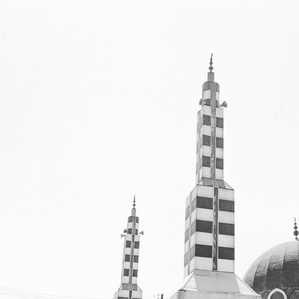
\includegraphics[width=0.4\linewidth]{captchas/1.png}
    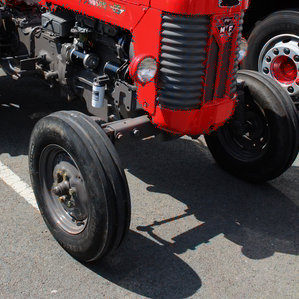
\includegraphics[width=0.4\linewidth]{captchas/2.png}
    \caption{Two CAPTCHA examples from Google where adversarial examples are used to fool web scrapers and spiders that are using automatic image classifiers such as DNNs.}\label{fig:googlecaptcha}
\end{figure}

Adversarial attacks can be classified as white-box and black-box depending on whether the attacker could reach the neural network parameters and gradients or not, respectively. Also, they can be classified as targeted or untargeted attacks. In targeted attack setup, there exists a particular class that attacker tries to modify the input image to have the attacked neural network to output that particular class and considered successful (or fooled the network) if the network outputs the target class when fed with the modified adversarial example. On the other hand, in the untargeted attack setting the attacker modifies the image to prevent the neural network from deciding the true class, which is the ground truth label of the input image and considered successful if the network outputs a class other than the true class label. In this thesis, targeted white-box attack setup is used. Other than the decision of the target network, there is often a magnitude constraint to the perturbation made and \(\mathcal{L}_p\) norms are widely used to measure the magnitude of the added perturbation. Adversarial attacks can be formally defined as a constrained optimization problem where the attacker tries to maximize a loss function by perturbing the input while the magnitude of the perturbation is constrained. Generally, the adversarial loss is the loss that is minimized throughout the training process. In most general form, the optimization process can be formulated as Equation \ref{eqn:somelabel}

\begin{equation}
    \label{eqn:somelabel}
    e=mc^2
\end{equation}

They also proposed a simple technique to generate adversarial examples called Fast Gradient Sign Method~(FGSM). It works by first calculating the gradient of the input with respect to a loss function, which is generally cross entropy loss

\section{Colorspaces}

\section{Perceptual Quality Preserving Adversarial Attacks}
Utilizing perceptual colorspaces and metrics for imperceptible adversarial example generation is investigated in several studies. Aksoy et al. investigated additive noise based attacks on chrominance channels in YUV colorspace \cite{aksoy2019attack}, which is the analog counterpart of \(YC_{b}C_{r}\) space. Despite Pestana et al. found that adversarial perturbations are more highlighted in luminance channels in terms of the magnitude~\cite{Pestana2020-hm}, Aksoy et al. found that even suppressing the luminance perturbation, additive noise based attack on chrominance channels still successfully fool target networks, yet causes visible distortion. In our earlier work, we also explored spatial transformations to UV channels of YUV to generate imperceptible adversarial examples~\cite{aydin2019imperceptible} and we extend this work by exploring \(YC_{b}C_{r}\) space as well as perceptually uniform CIELAB space and measuring structured similarity metrics such as SSIM~\cite{wang2004image} and MS-SSIM~\cite{wang2003multiscale} between benign images and adversarially generated images. Karli et al. leveraged perceptual metric LPIPS~\cite{zhang2018unreasonable} to improve the quality of adversarial examples. Since LPIPS is a differentiable metric, they used gradient based optimization to minimize LPIPS alongside the adversarial loss. Similarly, Zhao et al. replaced CIEDE2000 perceptual distance metric~\cite{luo2001development} with \(\mathcal{L}_{p}\) norm constraint in Carlini \& Wagner attack to produce perceptually close adversarial examples.

\section{Spatially Transformed Adversarial Examples}

Spatial transformations as a method for generating adversarial examples was first proposed in ~\cite{xiao2018spatially}, where it is shown that small displacements applied to input pixels can successfully fool a target network. However, using this method, even small displacements could cause visible distortions when the adjacent pixels are drifted towards different directions. As a remedy to this problem, use of  Total Variation~(TV) regularization~\cite{estrela2016total} was proposed. Application of TV regularization to the flow field pushes the neighboring displacement vectors to the same direction and, hence, produces smoother output. Similarly, Jordan et al. combined spatial transformations with \(l_\infty\) bounded attacks to forge stronger attacks with better perceptual quality. Croce et al. argued adding noise to smooth areas of an image causes visible artifacts and proposed "hiding" the perturbations at the locations with high spatial variations such as edges and corners~\cite{croce2019sparse}. As seen from Figure \ref{fig:diff}, perturbations made with our method naturally occurs in the places with high variations since it is based on local spatial transforms.



Unlike these methods, the attack proposed in this paper does not rely on auxiliary losses or explicit perceptual distance terms in optimization process to produce examples with high perceptual quality. In addition, it does not require regularization, unlike spatial transformation based methods such as ~\cite{xiao2018spatially}, due to its intrinsic imperceptibility. It should be noted that the existing spatial transformation based methods, as well as our work, does not utilize limited degree of freedom transformations such as rotation, translation or scaling that can be formulated as a \(4\times4\) transformation matrix~\cite{jaderberg2015spatial}. In that formulation, the flow field \(f \in \mathbb{R}^{2\times H \times W}\) is calculated using the transformation matrix. Instead, we directly define and optimize flow field, where the number of parameters is equal to twice number of pixels in the input image since there is an x and y component for each pixel. Application and optimization of flow field is explained in the Section \ref{chp:3_methodology}.

